% $File: main.tex
% $Date: Mon Jun 22 17:07:39 2015 +0800
% $Author: jiakai <jia.kai66@gmail.com>

\PassOptionsToPackage{bookmarksdepth=3}{hyperref}
\documentclass[bachelor]{thuthesis}
%\documentclass[master]{thuthesis}
%\documentclass[doctor]{thuthesis}
% \documentclass[%
%   bachelor|master|doctor|postdoctor, % mandatory option
%   secret,
%   openany|openright,
%   arialtoc,arialtitle]{thuthesis}

% 所有其它可能用到的包都统一放到这里了,可以根据自己的实际添加或者删除。
\usepackage{thutils}
\usepackage{pdfpages}
\usepackage{gensymb}
\usepackage{paralist}
\usepackage{metalogo}
\usepackage{scrextend}
../paper/mathdef.tex

% custom commands

\setcounter{tocdepth}{2}


% \textref{marker}{text}
\newcommand{\textref}[2]{\hyperref[#1]{#2}}
\newcommand{\figref}[1]{\hyperref[fig:#1]{\figurename~\ref*{fig:#1}}}
\newcommand{\tabref}[1]{\hyperref[tab:#1]{\tablename~\ref*{tab:#1}}}
\newcommand{\secref}[1]{\hyperref[sec:#1]{\ref*{sec:#1}节}}
\newcommand{\chapref}[1]{\hyperref[chap:#1]{第\ref*{chap:#1}章}}
\newcommand{\eqnref}[1]{\hyperref[eqn:#1]{(\ref*{eqn:#1})}}

% table lines
\newcommand{\tabtop}{\toprule[1.5pt]}
\newcommand{\tabmid}{\midrule[1pt]}
\newcommand{\tabbottom}{\bottomrule[1.5pt]}


% add plot
\newcommand{\addplot}[1]{\centering
    \includegraphics[width=0.85\textwidth,
    height=0.4\paperheight,keepaspectratio]{#1}}

\newcommand{\addtwocolplot}[2]{\centering
    \begin{minipage}{0.49\textwidth}
        \centering
        \includegraphics[width=\textwidth,
            height=0.4\paperheight,keepaspectratio]{#1}
    \end{minipage}
    \begin{minipage}{0.49\textwidth}
        \centering
        \includegraphics[width=\textwidth,
            height=0.4\paperheight,keepaspectratio]{#2}
    \end{minipage}
}
% single plot with two column size
\newcommand{\addplottcs}[1]{\centering
    \includegraphics[width=0.49\textwidth,
    height=0.4\paperheight,keepaspectratio]{#1}}


% 你可以在这里修改配置文件中的定义,导言区可以使用中文。
\def\myname{贾开}

\begin{document}


%%% 封面部分
\frontmatter

%%% Local Variables:
%%% mode: latex
%%% TeX-master: t
%%% End:
\secretlevel{绝密} \secretyear{2100}

\ctitle{基于非监督深度学习的医学影像特征提取研究}
% 根据自己的情况选,不用这样复杂
\makeatletter
\ifthu@bachelor\relax\else
  \ifthu@doctor
    \cdegree{工学博士}
  \else
    \ifthu@master
      \cdegree{工学硕士}
    \fi
  \fi
\fi
\makeatother


\cdepartment[计算机]{计算机科学与技术系}
\cmajor{计算机科学与技术}
\cauthor{贾开}
\csupervisor{宋亦旭~~副研究员}
% 如果没有副指导老师或者联合指导老师,把下面两行相应的删除即可。
%\cassosupervisor{陈文光教授}
%\ccosupervisor{某某某教授}
% 日期自动生成,如果你要自己写就改这个cdate
%\cdate{\CJKdigits{\the\year}年\CJKnumber{\the\month}月}

% 博士后部分
% \cfirstdiscipline{计算机科学与技术}
% \cseconddiscipline{系统结构}
% \postdoctordate{2009年7月——2011年7月}

\etitle{Research on Unsupervised Deep Feature Learning on Medical Images}
% 这块比较复杂,需要分情况讨论:
% 1. 学术型硕士
%    \edegree:必须为Master of Arts或Master of Science(注意大小写)
%              “哲学、文学、历史学、法学、教育学、艺术学门类,公共管理学科
%               填写Master of Arts,其它填写Master of Science”
%    \emajor:“获得一级学科授权的学科填写一级学科名称,其它填写二级学科名称”
% 2. 专业型硕士
%    \edegree:“填写专业学位英文名称全称”
%    \emajor:“工程硕士填写工程领域,其它专业学位不填写此项”
% 3. 学术型博士
%    \edegree:Doctor of Philosophy(注意大小写)
%    \emajor:“获得一级学科授权的学科填写一级学科名称,其它填写二级学科名称”
% 4. 专业型博士
%    \edegree:“填写专业学位英文名称全称”
%    \emajor:不填写此项
\edegree{Doctor of Engineering}
\emajor{Computer Science and Technology}
\eauthor{Kai Jia}
\esupervisor{Yixu Song}
%\eassosupervisor{Chen Wenguang}
% 这个日期也会自动生成,你要改么?
% \edate{December, 2005}

% 定义中英文摘要和关键字
\begin{cabstract}
    如何提取出兼具鲁棒性和区分性的特征是医学影像处理中的一个重要问题。
许多传统方法基于人工设计的浅层特征,无法在一般任务中达到足够的性能;
基于监督学习的方法依赖于对匹配点的人工标注;
而大部分非监督学习的方法又没有显式对特征应具有的不变性进行描述,
其性能没有根本保障。为了解决以上问题,
在本文中我们基于非监督学习的框架,
在深度卷积神经网络的损失函数里显式加入对特征鲁棒性和区分性的要求,
从而得到更好的特征提取器。同时我们提出了新的特征评测标准,
能在不通过其它图像处理任务来间接反映特征性能、
也不需要人工标注对应点的情况下,简明直接地完成对特征本身性能的评价。
实验结果证明我们的特征提取器优于之前的层叠卷积ISA,
这有望进一步提升许多医学影像处理算法的性能。

\end{cabstract}

\ckeywords{深度学习, 非监督学习, 特征提取, 医学影像处理, 卷积神经网络}

\begin{eabstract}
    hello, world
\end{eabstract}

\ekeywords{deep learning, unsupervised learning, liver image segmentation}

% 设置 PDF 文档的作者、主题等属性
\makeatletter
\thu@setup@pdfinfo
\makeatother
\makecover

% 目录
\tableofcontents


%%% 正文部分
\mainmatter
% $File: intro.tex
% $Date: Mon Jun 22 10:39:49 2015 +0800
% $Author: jiakai <jia.kai66@gmail.com>

\chapter{绪论\label{chap:intro}}

\section{研究背景}
对医学影像的获取、分析和处理在现代医疗工作中占有重要地位。
常用的基于放射的医学成像技术包括计算机体层成像(Computed Tomography, CT)、
磁共振成像(Magnetic Resonance Imaging, MRI)等。在医学影像技术的辅助下,
人们可以非侵入式的直接观察到患者体内的情况,
对疾病的诊治和人体科学的研究都有重大意义。

对医学影像的分析处理也是计算机科学相关领域长久以来研究的热点。
但由于其本身的难度以及对结果精确度的极高要求,这方面的自动化方法远不成熟,
只能作为人工辅助,临床上也一般由训练有素的医生来完成对影像的分析工作。
一般而言,医学影像的分析处理面临如下难点:
\begin{inparaenum}[(1)]
    \item 分辨率不高,如CT的图像矩阵往往只有$512\times 512$\cite{medimging2};
    \item 动态范围大,如CT值范围在$[-1000,1000]$Hu之间\cite{medimging2};
    \item 来源单一而封闭,需要大型扫描设备,而且涉及患者隐私;
    \item 由于人体构造、扫描时体位等不同而呈现很大差异性,
        病变部位则更是千差万别;
    \item 维度高,一般为3D体数据,或者带时间信息的4D图像。
\end{inparaenum}

许多医学影像或一般图像的处理算法并不直接处理原始图像数据,
而是先从原始图像上提取特征,再在特征空间上进行后续处理。
一般而言,特征提取包括检测关键点(或关键区域)和计算特征描述子两步,
在本文中我们着重于描述子的计算,并只考虑图像上逐点密集计算的特征描述子,
因此用``特征提取''一词代表计算特征描述子的过程。

图像处理中的特征提取指用低维的特征向量来描述高维的原始图像数据的过程。
原始图像数据一般包含大量冗余信息,例如相邻像素间差异的分布就往往集中于零点附近。
特征提取本质上就是对数据进行降维和去冗余,一个好的特征要能很好地描述原始图像,
应该同时具有鲁棒性和区分度。鲁棒性是指当原始图像经过平移、旋转、拉伸、亮度调整
等一些简单变换后,特征应该尽量不变;区分度是指对不同的图像,特征也应该尽量不同。

近年来随着互联网的高速发展带来的海量数据,
以及GPU技术的成熟和普及带来的高密度高速计算能力,
深度学习逐渐成为一种实用的高性能通用模型,并在图像分类\cite{he2015delving}、
人脸识别\cite{schroff2015facenet}等领域上取得飞跃发展,
乃至逼近甚至超过普通人类水平。
但目前将深度学习用于在医学影像上进行特征提取的工作并不多。因此,
本文将尝试使用基于非监督学习的深度学习算法,自动从CT扫描数据中提取特征,
并基于本文提出的评测方法测试各种特征的性能。

\section{研究现状}
学术界在特征提取、医学影像处理、深度学习等领域都有非常丰富的研究成果,
在本节中我们不会详细回顾所有的相关工作,
而仅仅对与本文密切相关的部分进行简要介绍。

在特征提取方面,有许多经典方法,大致可分为人工设计和非监督学习两大类。
人工设计的特征描述子,如LBP\cite{ojala1994performance}、
HOG\cite{dalal2005histograms}、SIFT\cite{lowe1999object}、
SURF\cite{bay2006surf}等,往往通过数学推导给特征引入所期望的不变性,
不会主动适配目标应用,不过在许多经典问题上都能取得不错的效果。
这些特征大部分是为2D图像设计的,也有少部分被扩展到了3D,
如3D-SIFT\cite{scovanner20073}。
非监督学习的特征描述子,可以主动适配到目标应用领域上,
有主成分分析、独立成分分析、独立子空间分析等统计方法,
也有受限玻尔兹曼机、自动编码器等可以学习深层特征的模型。
这方面的详细总结可以参考Bengio等人的总结\cite{bengio2013representation}。

需要指出的是,常见的非监督特征学习的方法往往基于概率模型。
其基本假设是使用少量参数对输入的概率分布$p(\vec{x})$进行建模,
如果该模型能较好地重建输入,则认为它提取了原始输入信息背后更本质的特征。
然而本文采取的方法并没有引入概率表述,而更类似判别学习的方法,
在监督信号中直接引入对鲁棒性和区分度的要求。
在这方面,与本文比较类似的是Dosovitskiy等人的工作
\cite{dosovitskiy2014discriminative},
其作者通过构建辅助分类来训练卷积神经网络并用于物体识别,
而在本文中我们除了多分类外还尝试了度量学习作为损失函数,
对训练数据量、特征距离度量等因素对性能的影响也进行了更详尽的探讨。

在医学影像处理方面,本文并没有大量涉及该领域相关的内容。
与本文比较相关的是Wu等人的工作\cite{wu2013unsupervised},
其作者使用层叠卷积ISA进行非监督特征学习,并用于人脑MRI扫描影像的配准。
但本文主要关注特征提取本身,并不使用具体的医学影像处理相关的任务来评价特征性能,
而是提出了新的特征评价标准。有了好的特征后,
一些传统的配准方法(如HAMMER\cite{shen2002hammer}、
多通道微分同胚demon\cite{peyrat2010registration})、
分割方法等都可能从中获益。

深度学习是近年来热门的研究领域。相关技术可用于监督学习、非监督学习等学习范式,
并用于供判别模型和生成模型。
关于深度学习更详细的讨论可以参考Bengio的总结\cite{bengio2009learning}。
本文采用深度卷积神经网络,其基本模型已在十多年前提出\cite{lecun1998gradient},
在近年来通过使用更深、更大的网络,更多的训练数据,
以及网络设计和训练过程中的一些技巧,这类模型在许多任务上都取得了不错的性能。


\section{主要贡献与创新点}
本文主要在以下几个方面作出了一定贡献:

\begin{enumerate}
    \item 实现了层叠卷积ISA方法\cite{wu2013unsupervised},
        并采用了多GPU的数据并行,极大提高了训练速度(
        相关代码已开源托管在\url{https://github.com/jia-kai/bachelor-thesis});
    \item 提出了新的特征评测标准,不需要依赖于特征在
        分割或配准等更复杂的任务上的表现来间接评价其性能,
        仅需要对某特定器官的分割标注作为额外输入,简明直接地评价特征性能;
    \item 在腹腔CT扫描影像上使用深度卷积神经网络进行非监督特征学习,
        基于我们的评测标准,通过实验证明其性能明显优于层叠卷积ISA方法,
        并且进行了细致的实验来比较训练过程中的各种参数选择对最终性能的影响,
        总结了提升网络性能的关键点。
\end{enumerate}

\section{论文组织}
本文的组织安排如下:

\chapref{intro}对研究背景、研究现状和本文的主要创新点进行了综述。

\chapref{ISA}介绍了层叠卷积ISA模型的基本原理及训练时的并行实现,
同时指出其缺陷以引出后续方法。

\chapref{CNN}介绍了本文所使用的深度卷积网络模型,
详细说明了其设计动机和损失函数的选择,并介绍了对3D影像数据进行增广的具体方法。

\chapref{expr}阐述了本文提出的特征评测方法,并给出了具体实验数据和结果的细节,
对实验结果进行了讨论。

\chapref{discuss}对本文的研究工作进行总结,并展望了未来的相关研究。

% vim: filetype=tex foldmethod=marker foldmarker=f{{{,f}}}

% $File: ISA.tex
% $Date: Tue Jun 09 16:07:31 2015 +0800
% $Author: jiakai <jia.kai66@gmail.com>

\chapter{基于层叠卷积ISA的特征提取\label{chap:ISA}}
本章主要介绍独立子空间分析(Independent Subspace Analysis, ISA)方法的基本原理,
及将其多次层叠后构成深度网络进行特征提取的方法,并对该方法进行简单的讨论。

\section{ISA的基本原理}
ISA是对独立成分分析(Independent Component Analysis, ICA)的扩展,
是一种经典的统计学习方法。
在本节中,先对ICA进行介绍,再将其扩展到ISA。关于ISA的更为详细的内容,
可以参考\cite{hyvarinen2009natural}。


\subsection{ICA的基本原理}
% f{{{
ICA是一种生成模型,其出发点是希望从对一个随机变量的一系列观察中,
分析出其背后的独立成分,每个成分有自己的概率分布,从而得出该随机变量的概率分布。

具体而言,对随机变量$\vec{x} = \trans{(x_1, \cdots, x_n)}$,ICA假设
\begin{eqnarray}
    \vec{x} = \vec{A}\vec{s}
    \label{eqn:ica:0}
\end{eqnarray}
其中,$\vec{A}$是一个$n\times m$的矩阵,$\vec{s}=\trans{(s_1,\cdots,s_m)}$
是一个$m$维随机变量,对于$i\neq j$,$s_i$和$s_j$独立。

实际应用时,一般$m \le n$,先对$\vec{x}$进行主成分分析(Principal Component
Analysis, PCA),降维成$m$维随机变量$\vec{z}=\vec{P}(\vec{x}-\bar{\vec{x}})$,
其中$\vec{P}$是$m \times n$的PCA矩阵;
另外\eqnref{ica:0}中的$\vec{x}$对应替换成$\vec{z}$,即
\begin{eqnarray}
    \vec{z} = \vec{B}\vec{s}
    \label{eqn:ica:1}
\end{eqnarray}
其中$\vec{B}$是$n\times n$矩阵,
用于将假设的独立特征空间变换到观察到的随机向量空间。显然\eqnref{ica:1}可逆,
记$\vec{B}^{-1}=\vec{V}$,有
\begin{eqnarray}
    \vec{s} = \vec{V}\vec{z}
    \label{eqn:ica:2}
\end{eqnarray}

在\eqnref{ica:0}中,$\vec{s}$解释了$\vec{x}$的概率分布,
可认为是一种更易处理、更能反应$\vec{x}$本质的特征;
而\eqnref{ica:2}则给出了从$\vec{x}$提取特征$\vec{s}$的方法,
其中$\vec{V}$就是特征检测器。

下面将简述基于最大似然来求解$\vec{V}$的方法。基于独立性的假设,有
\begin{eqnarray}
    \prob{\vec{s}} = \prod_{i=1}^m\prob[i]{s_i}
    \label{eqn:ica:3}
\end{eqnarray}
联合\eqnref{ica:2},于是有
\begin{eqnarray}
    \prob{\vec{z}} &=&  \prob{\vec{V}^{-1}\vec{s}} \nonumber \\
        &=& \abs{\det{\vec{V}}} \prob{\vec{s}} \nonumber \\
        &=& \abs{\det{\vec{V}}}\prod_{i=1}^m\prob[i]{s_i} \nonumber \\
        &=& \abs{\det{\vec{V}}}\prod_{i=1}^m\prob[i]{\trans{\vec{v_i}}\vec{z}}
    \label{eqn:ica:4}
\end{eqnarray}

假设对于$\vec{z}$有$T$个独立观测结果$\vec{z_1}\cdots\vec{z_T}$,
可定义最大似然为优化目标,于是ICA的参数$\vec{V}$估计如下:
\begin{eqnarray}
    \vec{V}^* &=& \argmax_{\vec{V}} L(\vec{V}) \nonumber \\
    &=& \argmax_{\vec{V}} \prod_{t=1}^T \prob{\vec{z_t}|\vec{V}} \nonumber \\
    &=& \argmax_{\vec{V}} \prod_{t=1}^T \left(\abs{\det{\vec{V}}}
            \prod_{i=1}^m\prob[i]{\trans{\vec{v_i}}\vec{z_t}} \right)
    \label{eqn:ica:5}
\end{eqnarray}

另外,由独立性,还应该要求$\vec{s}$的各分量不相关,即$\cov{\vec{s}} = \vec{I}$,
则需要$\vec{V}$满足$\trans{\vec{V}}\vec{V}=\vec{I}$,
于是有$\abs{\det{\vec{V}}}=1$,ICA的求解最终为如下形式:
\begin{eqnarray}
    \vec{V}^* &=& \argmax_{\vec{V}}
            \prod_{t=1}^T \left(
            \prod_{i=1}^m\prob[i]{\trans{\vec{v_i}}\vec{z_t}} \right) \nonumber
            \\
        \text{subject to} && \trans{\vec{V}}\vec{V}=\vec{I}
    \label{eqn:ica:6}
\end{eqnarray}

% f}}}

\subsection{扩展ICA到ISA}
% f{{{
从\eqnref{ica:2}得到的特征$\vec{s}$本质上是原始输入$\vec{x}$的线性变换。
线性变换的一个不足便是无法表达不变性,即输入发生任何改变,输出也都会对应变化,
无法对某些变换(如图像的小范围平移、旋转等)保持结果的稳定。

因此对ICA进行如下改进得到ISA:将特征$\vec{s}$分为$K$组,
第$k$组对应的分量下标集合记作$S(k)$。把每组特征看作一个子空间,
将其能量作为该子空间的特征输出。具体而言:
\begin{eqnarray}
    e_k = \sqrt{\sum_{i\in S(k)} s_i^2}
    \label{eqn:isa:0}
\end{eqnarray}

$\vec{e} = \trans{(e_1,\cdots,e_K)}$就是ISA最终的特征输出。

在ISA中,对$\vec{s}$各分量的独立性不做假设,而是假设$\vec{e}$的分量间独立,
并且仍然要求$\trans{\vec{V}}\vec{V}=\vec{I}$以得到尽量丰富的特征。
类似\eqnref{ica:6},基于最大似然对$\vec{V}$求解:
\begin{eqnarray}
    \vec{V}^* &=& \argmax_{\vec{V}}
            \prod_{t=1}^T \left(
            \prod_{k=1}^K\prob[k]{e_k} \right) \nonumber \\
        &=& \argmax_{\vec{V}}
            \prod_{t=1}^T \left(
            \prod_{k=1}^K\prob[k]{\sqrt{
                \sum_{i\in S(k)}\left(\trans{\vec{v_i}}\vec{z_t}\right)^2}
            }\right) \nonumber \\
        \text{subject to} && \trans{\vec{V}}\vec{V}=\vec{I}
    \label{eqn:isa:1}
\end{eqnarray}

一般而言,$p_k(s)$取为拉普拉斯分布(Laplace distribution),
即$p_k(s) = \frac{1}{2b}\exp(-\frac{\abs{s}}{b})$,
并在优化目标上取对数,最终ISA参数求解的形式如下:
\begin{eqnarray}
    L(V) &=& \sum_{t=1}^T \sum_{k=1}^K
        \sqrt{\sum_{i\in S(k)}\left(\trans{\vec{v_i}}\vec{z_t}\right)^2}
        \nonumber \\
    \vec{V}^* &=& \argmin_{\vec{V}} L(V) \nonumber \\
        \text{subject to} && \trans{\vec{V}}\vec{V}=\vec{I}
    \label{eqn:isa:opt}
\end{eqnarray}

而使用ISA提取特征的方法如下:
\begin{eqnarray}
    e_k &=&  \sqrt{\sum_{i\in S(k)} s_i^2} \nonumber \\
    \vec{s} &=& \vec{V}\vec{P}(\vec{x} - \bar{\vec{x}})
    \label{eqn:isa:extract}
\end{eqnarray}

% f}}}

\section{层叠卷积ISA\label{sec:isa:stacked-convolutional}}
% f{{{
以3D的CT扫描图像为例,要将ISA应用于图像处理,
一般是在扫描结果的数据里随机抽取$T$个$p\times p \times p$的图像小块,
把每个图像块平整化,看作一个$p^3$维的向量,将这些向量带入\eqnref{isa:opt}
求解参数$\vec{V}$。

处理图像数据时,ISA可以被放入卷积神经网络的框架中。
在\eqnref{isa:extract}中,
记$\vec{A} = \vec{V}\vec{P}$,$\vec{b}=-\vec{A}\bar{\vec{x}}$,
则$\vec{s}=\vec{A}\vec{x} + \vec{b}$可以看作一个全连接隐层输出。
记$\vec{A}$的维度是$m\times n$,而当$n=p^3$、
$\vec{x}$对应于一个$p\times p \times p$的图像块时,
$\vec{A}$可对应看作一个$m\times 1 \times p \times p \times p$的卷积核,
而其后的子空间的能量响应则可以看作是在多通道3D图像上进行的跨通道的非线性操作,
从而单层ISA可以看作由卷积以及非线性操作组成的卷积神经网络,
在这种框架下,单层的ISA可以被用于任意大小的输入图像上,
在图像上的每个点密集提取特征;在GPU的辅助下可以达到很高的速度。

但上述标准的单层ISA有两大缺点:
\begin{enumerate}
    \item 只有一层非线性,无法表达更高层更复杂的结构特征
    \item 由于优化过程中需要不断将权重矩阵正规化为正交阵,
        该过程复杂度为$\Theta(n^3)$,因此当输入图像块的维度较大时,
        训练会非常耗时。
\end{enumerate}

为了解决这两个问题,可以将多个这样的卷积ISA层叠起来,
从而作为一个深度特征提取器来使用。训练时可采取贪心逐层训练的方法,
在训练底层时使用较小的图像块,随后转换为卷积形式,
用较大的图像块作为输入并提取特征,在提取出的特征上再训练下一层ISA。
这种层叠卷积ISA的结构如\figref{isa:stack}所示。

\begin{figure}[H]
    \addplot{res/isa-stack.png}
    \caption{ISA及层叠卷积ISA对应的卷积神经网络结构\cite{wu2013unsupervised}}
    \label{fig:isa:stack}
\end{figure}

% f}}}

\section{训练方法及其实现}
% f{{{
为了优化\eqnref{isa:opt},我们使用带投影的整批梯度下降的方法。
先从均匀分布中随机采样得到初始权重矩阵$\vec{V_0}$;随后按如下规则迭代更新:
\begin{eqnarray}
    \vec{W_i} &=& \vec{V_{i-1}} - \alpha \frac{\partial L}{\partial
        \vec{V}}(\vec{V_{i-1}}) \nonumber  \\
        \vec{V_i} &=& \left(
            \vec{W_i}\trans{\vec{W_i}}\right)^{-\frac{1}{2}}\vec{W_i}
    \label{eqn:isa:train}
\end{eqnarray}
其中$\vec{W_i}$是沿梯度方向更新后的权重矩阵,而$\vec{V_i}$则是将$\vec{W_i}$
正规化使其成为正交阵。$\alpha$为学习速率,需要调整到合适的值使得$L(\vec{V_i})$
能较快下降而又不至于发生不稳定震荡。训练直到$L(\vec{V_i})$收敛才停止。

在实现方面,我们使用了theano\cite{bergstra+al:2010-scipy}作为训练框架,
用python实现训练功能。theano是一个符号计算框架,支持自动求导,
可以透明地实现GPU和CPU计算后端切换,同时内置了矩阵乘法、
卷积等各种常见操作的高效实现。

为了加速训练,我们实现了数据并行,可同时利用同一台主机上的多个GPU一起计算。
观察\eqnref{isa:opt}的损失函数$L(V)$,及\eqnref{isa:train}的更新规则,
可以发现在计算$\vec{W_i}$时很容易进行数据并行,
只需要将$T$个训练样本拆分成$N$份,各自求出的梯度相加后即可得到总体梯度,
然后再在CPU上更新$\vec{W_i}$及正规化得到$\vec{V_i}$。
这样单层的实际训练时间可以在半小时以内。


\subsection{对实现的简单验证}
在本小节中,我们通过简单的合成数据,来对ISA实现的正确性进行验证。
考虑各维服从独立高斯分布的40维随机变量$\vec{x}=\trans{(x_1,\cdots,x_{40})}$,
和各维服从独立均匀分布的10维随机变量$\vec{y}=\trans{(y_1, \cdots, y_{10})}$,
令
\begin{eqnarray}
    \vec{z} &=& \trans{(z_1, \cdots, z_{40})} \nonumber \\
    z_{4i+j} &=& x_{4i+j+1}y_{i+1} \nonumber \\
    && \forall 0 \le i \le 9,\,0 \le j \le 3
\end{eqnarray}

这样定义$\vec{z}$有两大好处,
一方面$\vec{z}$满足了ISA所需要的super-Gaussian分布,
另一方面将$\vec{z}$的各分量每4个分一组,则组内分量间也有了依赖性,
可以测试ISA的性能。采样$10000$个$\vec{z}$得到$40\times 10000$的矩阵$\vec{Z}$,
然后再从均匀分布中采样得到一个$64\times 40$的矩阵$\vec{M}$作为混合矩阵,
用$\vec{I} = \vec{M}\vec{Z}$作为最终呈现给ISA算法的输入。
为了评价ISA的效果,在求得ISA的权重矩阵$\vec{V}$后,
带入\eqnref{ica:2}中,然后计算$\corr{s_i^2, s_j^2}$作为$(i, j)$
处的元素绘制在\figref{isa:test}中,可以看出ISA能还原出这些随机变量间的内在结构,
被分在同一组的变量间也有较高的相关性。

\begin{figure}[H]
    \addplot{res/isa-toyeg.eps}
    \caption{在合成数据上ISA还原出的输入变量的内在关系}
    \label{fig:isa:test}
\end{figure}

% f}}}

\section{实验配置\label{sec:isa:expr}}
% f{{{
在本文中,均使用两层卷积ISA。第一层训练时输入的图像块大小为
$13\times 13 \times 13$,先用PCA把数据降维到$600$维,
每个子空间包含$2$个线性特征,输出维度为$300$维;
第二层的原始输入图像块大小为$21 \times 21 \times 21$,
先在图像块上以$8$为步长、用第一层卷积ISA得到$300$通道的$2\times 2 \times 2$
的图像块,共$2400$维作为第二层ISA训练的输入向量,PCA降维至$200$维,
子空间大小为$4$,最终输出特征维度为$50$维。

在SLIVER07的腹腔CT扫描数据上习得的第一层特征检测器如\figref{isa:filter}所示。
观察可以发现,其中很多都像检测各种朝向边缘的Gabor filter;
相邻两个检测器属于同一个子空间,可以看到它们的形态相似而在相位上有区别,
这也表明了一个子空间所对应的特征具有一定的平移不变性。

\begin{figure}[H]
    {
        \addplot{res/isa-filter.png}
        \caption{在实际数据上用ISA习得的第一层特征检测器}
        \label{fig:isa:filter}
    }
    \footnotesize
    图中展示了每个输出通道所对应的检测器,由于检测器本身是3D的,
    这里为了展示方便,仅选取了其中某一维的中间面片。
\end{figure}

% f}}}

\section{小结与讨论\label{sec:ISA:discuss}}
% f{{{
本节主要对ICA和ISA进行了介绍,描述了ISA到卷积神经网络的转化,并简述了训练方法。

ISA作为一种非监督学习的方法,其习得的特征可以自发的展现一定的平移和相位不变性
\cite{hyvarinen2000emergence}。
层叠卷积ISA被应用在了视频中的动作识别\cite{le2011learning}、
人脑MRI扫描图像的配准\cite{wu2013unsupervised}等领域,均取得不错的结果。

然而,叠卷积ISA也有一定的局限性:
\begin{enumerate}
    \item 卷积核大小需要与输入图像块的大小相同,使得对应的卷积核较大,
        而较大的卷积核会导致较慢的运行时间与较多的内存占用;
    \item 训练时采取贪心逐层训练的方法,缺乏全局优化的过程;
    \item 层数少,无法表达更复杂的结构,
        而且单层ISA的训练也要求输入向量维度不能太少,
        因此要想构造深层网络就需要很大的输入图像块;
    \item 最主要的一个缺陷是,ISA是一种完全非监督的方法;
        而实际应用中,我们往往希望特征对一定的平移、旋转等扰动具有不变性,
        这种要求无法整合进ISA的框架。
        虽然在实验中人们发现ISA习得的特征具有一定平移和相位不变性,
        可是对这种不变性的形式和程度都没有理论保障。
\end{enumerate}
% f}}}

% vim: filetype=tex foldmethod=marker foldmarker=f{{{,f}}}

% $File: CNN.tex
% $Date: Mon Jun 01 23:50:58 2015 +0800
% $Author: jiakai <jia.kai66@gmail.com>

\chapter{基于深度卷积神经网络的特征提取}
本章主要介绍基于深度卷积神经网络的特征提取方法。基于不同的损失函数,
本章提出两个模型,
但其基本思想都是针对\secref{ISA:discuss}提到的ISA方法的局限性,
通过人工构造的损失函数,引导网络学习出对仿射变换和Gamma校正有鲁棒性、
同时具有较强区分性的特征。

\section{网络结构}
深度卷积神经网络一般由卷积、池化、全连接等层组成,
卷积和全连接层后一般接一个非线性函数。在本小节中,
先对这三种层对应的数学操作进行介绍,随后再给出本文所用的网络结构。

\subsection{基本数学操作}


\subsection{本文所用网络结构}
本文仅试验了一种网络结构,其计算层由三层卷积、一层池化、两层全连接组成。
为了与\secref{isa:expr}所描述的ISA模型公平比较,
输入与之相同用$21\times 21 \times 21$的图像块,输出同样为$50$维特征。
图像块在进入网络之前,
先要经过线性变换$\vec{y}=k\vec{x}+b$,其中$k$、$b$为在训练集上求得的标量常数,
使得$E[\vec{y}]=0$,$\max(\abs{\vec{y}})=1$。
网络中所有卷积和全连接层均使用使用ReLU作为非线性,即$f(x)=\max(x, 0)$。
具体的网络结构参数见\tabref{cnn:arch}。

\begin{table}[h!]
    \begin{center}
        \caption{本文所用的深度卷积神经网络结构}
        \label{tab:cnn:arch}
        \begin{tabular}{c|c|c}
            \hline
            {\heiti 层编号} & {\heiti 输入大小} & {\heiti 层内容} \\ \hline
            0 & $1\times 21 \times 21  \times 21$ & 线性变换:$y=kx+b$ \\
            1 & $1\times 21 \times 21  \times 21$ & $Conv(20, 4)$ \\
            2 & $20\times 18 \times 18  \times 18$ & $MeanPooling(2)$ \\
            3 & $20\times 9 \times 9 \times 9$ & $Conv(24, 4)$ \\
            4 & $24\times 6 \times 6 \times 6$ & $Conv(28, 4)$ \\
            5 & $28\times 3 \times 3 \times 3$ & $FC(60)$ \\
            6 & $60$ & $FC(50)$ \\
            7 & $50$ & 损失函数 \\
        \end{tabular}
    \end{center}
    \footnotesize
    注:
    \begin{center}
        \begin{itemize}
            \item $Conv(c, s)$ 表示输出通道数为$c$,
                卷积核大小为$s\times s \times s$,
                步长为$1$的3D卷积
            \item $MeanPooling(s)$ 表示大小为$s\times s \times s$
                且无重叠的均值池化
            \item $FC(n)$ 表示输出维度为$n$的全连接层
        \end{itemize}
    \end{center}
\end{table}

\section{损失函数}
\subsection{分类输出:Softmax与交叉熵损失函数}
\subsection{特征输出:度量学习}

\section{数据增广}
简要形式化描述希望特征对变换$F(A, \gamma)=(affine(A), gamma(\gamma))$
满足的不变性

\subsection{Gamma校正}

\subsection{三维仿射变换}

\section{训练方法}

% vim: filetype=tex foldmethod=marker foldmarker=f{{{,f}}}


% $File: expr.tex
% $Date: Fri Jun 12 16:10:59 2015 +0800
% $Author: jiakai <jia.kai66@gmail.com>

\chapter{评测方法与实验\label{chap:expr}}
本章首先提出一种评测方法,其完全基于对某器官的分割标注,
无需依赖其它图像处理任务来间接反映特征性能,
也无需显式计算两个标注间的点对应关系,
可以直接评价特征本身的优劣。随后本章介绍实验所用数据集,
并报告基于该评测方法的实验结果。

\section{评测方法}
% f{{{
在实际应用中,往往难以有单一可靠的方法直接评判特征优劣,
而是需要有一个依赖某特征的具体任务,
并通过该特征在该任务上的表现来间接反应特征优劣。
例如,SIFT特征最早被用于物体识别\cite{lowe1999object},
层叠卷积ISA被用于动作识别\cite{le2011learning}、
大脑MRI扫描的柔性配准\cite{wu2013unsupervised}等。
然而,如果任务过于复杂,
结果往往会受到任务相关的具体算法的影响。
例如在Guorong Wu的工作\cite{wu2013unsupervised}中,
作者的评测过程依赖于第三方软件的预处理,
而且发现换用ISA特征后在Demons算法上的配准性能反而变差了,
虽然作者表示这是由于实验过程带来的一些不公平造成的,
但客观而言在这种复杂的环境下确实更难分离出特征本身在最终性能里的贡献。
因此,在本节中,我们将提出一个新的简单而普适的方法来评测特征性能,
以免结果受到过于复杂的任务相关算法的影响。
简单而言,该方法基于人工标定的器官分割掩膜,在不需要具体点对应关系的情况下,
通过在我们定义的边界距离上的匹配精确度,
来衡量特征的性能。

\subsection{基于器官分割标注的曲面匹配}
我们的评测方法要求数据提供对某个器官的分割标注,
例如在本文中我们使用SLIVER07中的肝脏分割标注。
在本小节中,我们将介绍基于大量带器官分割标注的训练数据,
在单个测试图像上寻找某个曲面的方法。为此,我们先定义单点匹配,
并将其扩展到曲面。

\subsubsection{单点匹配}
基于分割标注,我们对每个点都定义{\bf 边界距离},
并基于边界距离来判断单点是否匹配成功。

我们假设器官分割掩膜以二值3D图像$\vec{M}$的形式提供,
$\vec{M}$中某点值为$1$时表示对应点属于目标器官,为$0$时表示不属于目标器官。
对于每个点$(i, j, k)$,定义
\begin{eqnarray}
    N(i, j, k) &=& \prod_{
        \max(\abs{x}, \abs{y}, \abs{z}) = 1}
        M(i + x, j + y, k + z)
\end{eqnarray}
$N(i, j, k)$表示了与$(i, j, k)$相邻的点中是否有不属于目标器官的点。
于是可定义边界点集为:
\begin{eqnarray}
    \partial M &=& \left\{\,\vec{p} : M(\vec{p}) = 1\,\text{且}\,
        N(\vec{p}) = 0\,\right\}
\end{eqnarray}

把每个点看作无向图的顶点,同时在几何上看作一个单位立方体,
对于有公共顶点或公共边的两点间连一条权值为$1$的边,
于是对任意两点$\vec{p}, \vec{q}$,其间存在最短路,
距离记作$s(\vec{p}, \vec{q})$。
对每个点$\vec{p}$,可定义无符号边界距离$D(\vec{p})$和边界距离$d(\vec{p})$:
\begin{eqnarray}
    D(\vec{p}) &=& \min_{\vec{q} \in \partial M} s(\vec{p}, \vec{q})
        \nonumber \\
    d(\vec{p}) &=& (2M(\vec{p})-1)D(\vec{p})
\end{eqnarray}
在涉及多个图像如$\vec{M_1}$、$\vec{M_2}$时,
我们通过脚注形式来区分各自的边界距离:
$d_{\vec{M_1}}(\vec{p})$、$d_{\vec{M_2}}(\vec{q})$。

对于参考图像$\vec{R}$上的某点$\vec{p}$及其特征$\vec{f(p)}$,
我们在测试图像$\vec{T}$上寻找特征距离最小的点$\vec{q}$,
称$\vec{q}$为$\vec{p}$的匹配点,
如果还有$\abs{d_{\vec{R}}(\vec{p}) - d_{\vec{T}}(\vec{q})} \le \theta$,
则认为匹配成功,其中$\theta$为容忍的距离误差,本文中均取$1$。
为了在特征上快速、精确地寻找匹配点,即特征空间上的最近邻,
我们把两两特征间的距离计算转换成矩阵乘法并在GPU上运行。

为了确保这种基于边界距离的匹配验证方法的准确性,
我们在所有数据的数十万成功匹配点对中随机抽取了50对
并绘制在\figref{expr:pt:match}中,
人工观察可以发现,评测算法所认为成功匹配的点对,
大部分确实是真实匹配的。
\begin{figure}[h!]
    {
        \addplot{res/expr-match/pt-patch.png} \\
        \vspace{0.2em}
        \addplot{res/expr-match/pt-bd-dist.png}
        \caption{成功匹配点对的抽样观察}
        \label{fig:expr:pt:match}
    }
    \footnotesize
    上半部分为以匹配点对为中心的周边图像块,
    为了便于人工观察,我们将一部分输入周边区域也绘制在这里,
    其中中心绿色部分为特征提取器实际的输入。
    我们单独将每对匹配图像块的灰度值线性归一化到$[0, 255]$区间以便显示。 \\
    下半部分为根据肝脏分割标注计算出的边界距离,
    为了便于观察这里使用无符号距离,纯白表示距离为$0$,颜色越深则距离越大。
\end{figure}

\subsubsection{曲面匹配\label{sec:expr:match}}
上述单点匹配的判别方法,易受各种随机因素的影响,
在这里我们将其扩展到曲面匹配以提高鲁棒性。

首先根据边界距离,对器官分割标注$\vec{M}$定义参考曲面:
\begin{eqnarray}
    \hat{\vec{M}} &=& \left\{ \vec{p} : d_{\vec{M}}(\vec{p}) = d_0 \right\}
\end{eqnarray}
在本文中,取参考曲面为边界稍靠内的曲面,取$d_0=2$,
这样的一个好处是所有可能成功匹配的点的边界距离在$[1, 3]$间,
于是也都在目标器官内部靠近边界处。

假设我们有$N$个训练数据$\vec{M_1},\cdots,\vec{M_N}$,
我们在$\hat{\vec{M_1}},\cdots,\hat{\vec{M_N}}$上各均匀选取$T$个点,
并在测试图像的上寻找这$NT$个点的匹配点。
为了防止特征只注重了很明显的局部特点而导致匹配点过于集中,
我们把测试图像分成了若干个小方格,每个的大小为$k\times k \times k$,
对于落入同一方格的匹配点,只保留其中距离最小的点,
匹配精确度定义为这些剩下的点中成功匹配的点数占剩下的点总数的比例。
在本文的实验中,均取$T=3000, k=2$。


\subsection{ROC曲线}
基于\secref{expr:match}中针对单个测试图像的曲面匹配方法,
在本小节中我们给出其ROC曲线绘制的方法,以及多个测试图像的整体评分方法。

假设有$M$个测试图像,固定特征距离阈值$\theta$,对每个测试图像,
仅保留$\theta$以下的匹配点,则此时可以得到$(t_1^{(\theta)},
a_1^{(\theta)}),\cdots,(t_M^{(\theta)}, a_M^{(\theta)})$共$M$个二元组,
$t_i^{(\theta)}$表示这些匹配点占所有训练图像的参考曲面上选中的点的比例,
沿用上节记号,则这些选中的点的总数为$NT$,
$t_i^{(\theta)}$就是$\theta$限制下总匹配点数与$NT$之商,
反映了匹配的稀疏程度;
$a_i^{(\theta)}$表示所有训练图像在第$i$个测试图像上
特征距离不超过$\theta$的匹配点中成功匹配的比例,即$\theta$限制下的匹配精确度。
记$t^{(\theta)}$为$\{t_1^{(\theta)},\cdots,t_M^{(\theta)}\}$的均值,
$a^{(\theta)}$、$s^{(\theta)}$分别为
$\{a_1^{(\theta)},\cdots,a_M^{(\theta)}\}$的均值和方差,
显然$t^{(\theta)}$随着$\theta$增加是单调不下降的。
遍历$\theta$取值,
将所有$(t^{(\theta)}, a^{(\theta)})$对应的平面点连接起来,
就得到了ROC曲线,
同时可以作出$a^{(\theta)} \pm s^{(\theta)}$的对应区域来反应评测的准确度。
在本文的ROC曲线中,我们把$a^{(\theta)}$称为精确度(precision),
$t^{(\theta)}$称为顶峰比(top ratio)。

\figref{expr:match}展示了在阈值限制下匹配点分布的变化。
可以发现,当限制阈值后,输出的都是该模型比较确信的点,
这些点更靠近如肝肺交界处等有强边缘特征的区域,
匹配精确度能有较大提高。
为了防止顶峰比较低时仅考虑集中于强边缘区域的匹配点而影响对整体性能评价,
我们仅考虑顶峰比在区间$[0.05, 1]$范围内的曲线。

\figref{expr:curve:ISA}给出了一条这样的ROC曲线,
其中每个线条后的半透明背景反映了$s^{(\theta)}$的大小;
曲线上的点均来自$(t^{(\theta)}, a^{(\theta)})$的原始值,
相邻两点间线性插值,每条曲线使用$10000$个点绘制。
比较两条曲线时,精确度越高、精确度的方差越小、
顶峰比越高,则对应的特征的性能越好。
为了直接比较两条曲线,我们可以用AUC(Area Under Curve, 曲线下面积)
及平均精确度两个指标。
AUC定义为曲线的精确度对顶峰比的定积分值,
平均精确度为AUC除以顶峰比的最大、最小值之差。
在本文的ROC曲线中,各曲线名称后的括号里注明的数字是平均精确度。

\begin{figure}[h!]
    {
        \addplot{res/expr-match/48.2.png} \\
        \vspace{0.2em}
        \addplot{res/expr-match/80.1.png}
        \caption{限制阈值导致匹配点分布的变化}
        \label{fig:expr:match}
    }
    \footnotesize
    这两张图均通过在某扫描轴上按4像素为步长切片绘制。
    其中彩色标注的区域是人工标注的肝脏区域,绿色点为成功匹配点,
    蓝色点为失败匹配点,蓝色、绿色颜色越亮,则表示匹配的特征距离越小。
    为方便查看,每个点用原始点为中心的$5\times 5 \times 5$立方体来表示,
    因此在某些切片上的一些成功匹配点看起来离参考曲面很远,
    其实是来自曲率变化剧烈的区域的其它(未在此绘制的)切片。

    上图绘制了所有匹配点,顶峰比为$0.568$,匹配精确度为$48.2\%$;
    下图限制了阈值,顶峰比为$0.078$,匹配精确度为$80.1\%$。
\end{figure}

% f}}}

\section{实验数据集}
% f{{{
本文的实验均采用SLIVER07\cite{heimann2009comparison}
所提供的腹腔CT扫描数据及肝脏标注。
SLIVER07是一次肝脏分割的比赛,提供了20个训练数据,
由于数据损坏等原因我们仅成功解压出其中的18个数据,
并随机选取其中12个作为训练数据,6个作为测试数据。
先对这18个数据按如下步骤预处理:
\begin{enumerate}
    \item 按数据中给出的CT扫描时各轴的空间间隔构造不等比拉伸的仿射变换矩阵,
        对图像进行仿射变化,使得各个方向上每个像素对应的空间尺度相同;
    \item 将图像缩小至$0.8$倍;
    \item 计算肝脏分割标注的包围盒(即最小的可完全包含每个标注点的立方体),
        将包围盒向外扩大$1.2$倍,必要时继续扩大以保证包围盒边界到标注点的最近距
        离不少于11个像素,裁剪出该范围内的图像作为预处理过的图像。
\end{enumerate}
其中后两步的目的主要是减小图像尺寸,以加速训练和测试。

训练数据均随机采自预处理过的图像。随机采样时,确保以下两点以保证采样质量:
\begin{enumerate}
    \item 新采样的图像块和当前图像上已采样的图像块的重合部分的体积不超过$0.5$
        倍图像块体积;
    \item 采得的图像块要有一定的平均亮度,且灰度值变化范围要超过一定阈值。
\end{enumerate}

在训练深度卷积神经网络时,Gamma变化的范围是$[0.7, 1.4]$,
仿射变换的最大平移量为$1.2$像素,最大旋转角度为$35\degree$,
拉伸范围是$[0.8, 1.2]$。

% f}}}

\section{实验结果与讨论}
% f{{{
在本节中,我们将展示并讨论具体的实验结果。为了进行特征匹配,
首先需要明确特征距离的度量方法,在本文中我们测试了如下两种度量方法。

曲线名称以-cos结尾的表示使用余弦距离:
\begin{eqnarray}
    d_{\cos}(\vec{x}, \vec{y}) &=& 1 -
        \frac{\trans{\vec{x}}\vec{y}}{\abs{\vec{x}}\abs{\vec{y}}}
\end{eqnarray}

曲线名称以-$L_2$结尾的表示使用欧式距离:
\begin{eqnarray}
    d_{L_2}(\vec{x}, \vec{y}) &=&
        \trans{(\vec{x}-\vec{y})}(\vec{x}-\vec{y}) \nonumber \\
        &=& \trans{\vec{x}}\vec{x} + \trans{\vec{y}}\vec{y} -
        2\trans{\vec{x}}\vec{y}
\end{eqnarray}

需要指出的是,基于余弦距离定义的全序关系
等价于把向量投影到单位超球面后再按欧氏距离定义全序关系。

\subsection{基于层叠卷积ISA的特征提取\label{sec:expr:isa}}
对于层叠卷积ISA方法,我们从每个被试的扫描影响上随机取$50000$个图像块,
并按照\chapref{ISA}中介绍的方法进行训练。
最终在测试集上的ROC曲线如\figref{expr:curve:ISA}所示。

可以发现,使用余弦距离测度的情况下,在较低顶峰比时的精确度显著提高,
说明在余弦距离下特征的测度更有意义,可以根据距离的值来反应对匹配精确度的信心。
所以,如果要使用层叠卷积ISA的特征进行大规模图像块的匹配,
应该先把特征归一化到单位长度再建立空间索引数据结构。

\begin{figure}[h!]
    \addplot{res/expr/isa.pdf}
    \caption{ISA的ROC曲线}
    \label{fig:expr:curve:ISA}
\end{figure}

\subsection{基于多分类进行特征学习的深度卷积神经网络\label{sec:expr:clsfy}}
对于\secref{cnn:loss:clsfy}中介绍的基于多分类监督信号来进行间接特征学习的方法,
我们尝试了不同的训练数据量,均使用带Nesterov momentum的SGD算法
\cite{sutskever2013importance}进行优化,momentum设置为$0.95$。
训练过程中如果发现损失函数的值在最近$5$轮中有$2$次增长,
则将学习速率减少到原来的$0.92$倍;学习速率减少到$10^{-8}$时停止训练。
在本小节中,我们将比较不同的参数选择对基于多分类训练的网络所提取特征性能的影响。
关于曲线命名的具体法则,见\secref{expr:allresults}。

\subsubsection{距离度量}
我们测试了用余弦距离和欧式距离度量特征相似度,
结果如\figref{expr:curve:clsfy:measure}所示,
可以看出在大部分情况下,采用欧式距离时精确度更好。

\begin{figure}[h!]
    \addtwocolplot{res/expr/clsfy/measure/0.pdf}{res/expr/clsfy/measure/1.pdf}
    \addtwocolplot{res/expr/clsfy/measure/2.pdf}{res/expr/clsfy/measure/3.pdf}
    \addplottcs{res/expr/clsfy/measure/4.pdf}
    \caption{基于多分类的深度卷积神经网络的特征在不同距离度量下的性能}
    \label{fig:expr:curve:clsfy:measure}
\end{figure}

\subsubsection{训练数据量}
\secref{cnn:discuss}中已经提到,
这种基于多分类的训练方法要求训练数据中没有来自不同被试、但
对应于同一解剖学位置的图像块,否则可能会使得模型过度关注个体特征导致性能下降。
我们实验了在各被试上分别采集$200$、$400$、$800$、$2000$、$5000$
个图像块作为训练数据,其各自性能如\figref{expr:curve:clsfy:datasize}所示。
\begin{figure}[h!]
    \addplot{res/expr/clsfy/datasize.pdf}
    \caption{训练数据量对多分类学习的深度卷积神经网络的性能影响}
    \label{fig:expr:curve:clsfy:datasize}
\end{figure}

可以看出,实验结果支持我们的观点,
在每个被试的扫描数据中采集$400$个图像块时性能最好,
过多或过少均会导致性能下降,当数量过多时性能下降更为明显。

\subsubsection{结合PCA进一步提升性能\label{sec:expr:clsfy:pca}}
在实验中我们还发现,去掉最后一层全连接,即\tabref{cnn:arch}中的第6层之后,
用一个从$60$维降维到$50$维的PCA代替该全连接层,可以进一步提升网络的性能。
求解该PCA层的权重时所用的数据来自每个被试上随机采集$10000$个图像块得到的数据。
与\secref{expr:isa}中的发现类似,使用PCA特征时,用余弦距离效果更好。
具体ROC曲线如\figref{expr:curve:clsfy:pca}所示。

\begin{figure}[h!]
    \centering
    \addtwocolplot{res/expr/clsfy/pca/0.pdf}{res/expr/clsfy/pca/1.pdf}
    \caption{结合PCA提升多分类训练的深度卷积神经网络的特征性能}
    \label{fig:expr:curve:clsfy:pca}
\end{figure}


\subsection{基于度量学习进行特征学习的深度卷积神经网络}
我们采用了Adam\cite{kingma2014adam}来优化\secref{cnn:loss:mtrc}中定义的网络,
因为实验中我们发现其优化效果比SGD更好。与\secref{expr:clsfy}类似,
当学习速率自动下降到一定程度后停止训练。
在本小节中,我们将比较不同的参数选择对基于度量学习的网络所提取特征性能的影响。
关于曲线命名的具体法则,见\secref{expr:allresults}。

\subsubsection{距离度量}
由于训练时就直接使用了余弦距离,在测试时,
余弦距离的性能也应该比欧氏距离更好。
如\figref{expr:curve:mtrc:measure}所示,使用余弦距离时精确度的方差更小,
精确度普遍更高,而且最终顶峰比也更高。

\begin{figure}[h!]
    \addtwocolplot{res/expr/mtrc/measure/0-0.pdf}{res/expr/mtrc/measure/0-1.pdf}
    \addtwocolplot{res/expr/mtrc/measure/1-0.pdf}{res/expr/mtrc/measure/1-1.pdf}
    \addtwocolplot{res/expr/mtrc/measure/2-0.pdf}{res/expr/mtrc/measure/2-1.pdf}
    \caption{基于度量学习的深度卷积神经网络的特征在不同距离度量下的性能}
    \label{fig:expr:curve:mtrc:measure}
\end{figure}

\subsubsection{损失函数中的$\delta$}
\eqnref{cnn:mtrc:loss}中用到了一个超参数$\delta$来控制对不同类的特征应有的距离。
我们实验了$\delta=0.5$和$\delta=0.65$两种设定,
发现虽然较大的$\delta$可以在训练集上让类内距离减小而类间距离增加,
但在测试集上却让性能有所下降。因此,控制$\delta$的值,
可以在一定程度上减轻过拟合。具体ROC曲线如\figref{expr:curve:mtrc:delta}所示,
其中带-mg的曲线表示使用了$\delta=0.65$。

\begin{figure}[h!]
    \addtwocolplot{res/expr/mtrc/delta/0.pdf}{res/expr/mtrc/delta/1.pdf}
    \addplottcs{res/expr/mtrc/delta/2.pdf}
    \caption{$\delta$对度量学习的深度卷积神经网络的性能影响}
    \label{fig:expr:curve:mtrc:delta}
\end{figure}

\subsubsection{训练数据量}
我们也测试了不同训练数据量对最终性能的影响,发现数据量达到一定程度后,
并不会对最终性能产生太大影响,这也与预期相符。
ROC曲线见\figref{expr:curve:mtrc:datasize}。
\begin{figure}[h!]
    \addtwocolplot{res/expr/mtrc/datasize/0.pdf}{res/expr/mtrc/datasize/1.pdf}
    \caption{训练数据量对度量学习的深度卷积神经网络的性能影响}
    \label{fig:expr:curve:mtrc:datasize}
\end{figure}

\subsubsection{结合PCA进一步提升性能}
与\secref{expr:clsfy:pca}中讨论的方法类似,
我们可以用PCA替代最后一层全连接来提升特征的性能。
然而我们发现,对某些网络,倒数第二层的一些神经元由于偏置量太大而始终没被激活,
导致PCA时协方差矩阵的很多特征值(eigenvalue)几乎为$0$,无法实现$50$维的PCA输出。
我们限制了PCA时最小特征值不小于$0.1$,并依此决定最终PCA的输出维度。
ROC曲线见\figref{expr:curve:mtrc:pca}。
\begin{figure}[h!]
    \addtwocolplot{res/expr/mtrc/pca/0.pdf}{res/expr/mtrc/pca/1.pdf}
    \addtwocolplot{res/expr/mtrc/pca/2.pdf}{res/expr/mtrc/pca/3.pdf}
    \caption{结合PCA提升度量学习的深度卷积神经网络的特征性能}
    \label{fig:expr:curve:mtrc:pca}
\end{figure}

\subsection{对特征距离及ROC曲线形态的讨论}
一般情况下随着阈值与顶峰比的提高,
错误匹配点对数量比成功匹配点对数量增加地更快,所以匹配精确度应该下降,
ROC曲线应该是下降曲线;
但实验中少数曲线却与此相反,
\figref{expr:curve:ISA}中ISA在欧氏距离下的ROC曲线
和\figref{expr:curve:clsfy:measure}中多分类学习的网络在$5000$采样密度时的ROC曲线
尤为特别。我们认为其原因是,特征性能较差,即使用不合理的距离度量、
或者网络产生的特征本身就不合理时,
大量成功匹配点对间距离反而比错误匹配的点对间距离更大,
也就是说这里的距离无法反映模型对匹配正确率的信心。
为了验证该想法,我们在\figref{expr:curve:border-dist-stat}
中绘制了匹配点的边界距离与特征距离的关系。
在图中除了前述的趋势特别的曲线外,
我们还绘制了性能较好的特征所对应的曲线。
可以看出,当特征性能较好时,对于成功匹配的点,特征距离也较小,
在这种情况下特征距离可以作为对匹配准确度信心的反映;
而如果特征距离无法反映对成功匹配的信心,那么特征的性能也往往较差。
另外在实际应用中,要想提高匹配精度,可以限制特征距离的最大值,
当然代价就是总匹配点对的数量也会相应减少。

\begin{figure}[h!]
    {
        \addtwocolplot{res/expr/border-dist-stat/l2.pdf}{res/expr/border-dist-stat/cos.pdf}
        \caption{匹配点的边界距离与特征距离的关系}
        \label{fig:expr:curve:border-dist-stat}
    }
    \footnotesize
    绘制方法是将所有匹配点对按其在测试图像上的边界距离分组,
    每组的边界距离作为横坐标,每组内所有点的平均特征距离作为纵坐标。
    图中浅红背景的纵向区间标记了成功匹配所要求的边界距离范围,即$[1, 3]$。
    另外,由于我们关心的是特征距离间的相对大小,在这里为了展示方便,
    每条曲线的特征距离都被线性缩放到$[0, 1]$区间内。
\end{figure}


\subsection{结果汇总\label{sec:expr:allresults}}
在本小结中,我们将汇总所有结果,以备参考。

首先介绍结果命名规则。所有结果按照``方法名-[参数0-][参数1-]...距离度量''
的形式命名。距离度量包括cos和$L_2$,分别代表余弦距离和欧氏距离。
方法名包括ISA、clsfy、mtrc,分别代表层叠卷积ISA、
基于多分类或度量学习训练的深度卷积神经网络。
对于后两种方法,还有如下额外参数:
\begin{description}
    \item[d$N$] 表示训练数据量为从每个被试上随机采样$N$个图像块
    \item[mg] 表示基于度量学习的方法使用了$\delta=0.65$
    \item[pca] 表示使用了PCA代替最后一层全连接
    \item[o$N$] 表示最终特征维度不是$50$维,而是$N$维
\end{description}

我们将各类方法中,结果最好的ROC曲线共同绘制在\figref{expr:curve:all}里,
以便比较。为了便于观察,该图中没有绘制方差范围。

\begin{figure}[h!]
    \addplot{res/expr/all.pdf}
    \caption{ROC曲线汇总}
    \label{fig:expr:curve:all}
\end{figure}

另外,我们将所有实验结果的一些统计数据放在\tabref{expr:all}中。
其中括号内标注的是按该列统计值的排名,前三名加粗标注。
\begin{longtable}{l|l|l|l|l|l}
    \caption{全部实验结果}
    \label{tab:expr:all} \\
    \tabtop
    {\heiti 名称} & {\heiti AUC} & {\heiti 平均精确度} & {\heiti 最大顶峰比} &
        {\heiti 最小精确度} & {\heiti 最大精确度} \\
    \tabmid
    ISA-cos&0.218 (25)&0.349 (32)&$\boldsymbol{0.674}$ {\bf (1)}&0.235 (33)&0.543 (28)\\
ISA-l2&0.122 (35)&0.212 (35)&$\boldsymbol{0.629}$ {\bf (2)}&0.179 (34)&0.227 (36)\\
clsfy-d200-cos&0.246 (18)&0.555 (12)&0.493 (29)&0.399 (19)&0.782 (7)\\
clsfy-d200-l2&0.247 (17)&0.571 (9)&0.483 (31)&0.405 (15)&0.788 (5)\\
clsfy-d400-cos&0.259 (14)&0.551 (13)&0.521 (25)&0.402 (16)&0.774 (8)\\
clsfy-d400-l2&0.264 (10)&0.583 (5)&0.503 (28)&0.418 (12)&$\boldsymbol{0.801}$ {\bf (3)}\\
clsfy-d400-pca-cos&$\boldsymbol{0.293}$ {\bf (2)}&0.598 (4)&0.540 (19)&0.426 (9)&$\boldsymbol{0.830}$ {\bf (1)}\\
clsfy-d400-pca-l2&0.263 (11)&0.562 (10)&0.518 (26)&0.445 (4)&0.735 (13)\\
clsfy-d800-cos&0.213 (26)&0.433 (28)&0.542 (18)&0.333 (29)&0.611 (22)\\
clsfy-d800-l2&0.241 (20)&0.501 (19)&0.530 (21)&0.350 (26)&0.738 (12)\\
clsfy-d800-pca-cos&0.275 (7)&0.523 (16)&0.575 (8)&0.364 (24)&0.755 (10)\\
clsfy-d800-pca-l2&0.228 (22)&0.461 (25)&0.545 (16)&0.365 (23)&0.644 (20)\\
clsfy-d2000-cos&0.156 (33)&0.313 (33)&0.548 (14)&0.266 (32)&0.363 (33)\\
clsfy-d2000-l2&0.178 (32)&0.357 (31)&0.550 (13)&0.267 (31)&0.422 (32)\\
clsfy-d5000-cos&0.125 (34)&0.223 (34)&0.611 (4)&0.095 (35)&0.245 (35)\\
clsfy-d5000-l2&0.118 (36)&0.209 (36)&$\boldsymbol{0.616}$ {\bf (3)}&0.094 (36)&0.249 (34)\\
mtrc-d800-cos&0.274 (8)&0.520 (17)&0.577 (7)&0.359 (25)&0.729 (14)\\
mtrc-d800-l2&0.206 (28)&0.398 (29)&0.567 (12)&0.343 (27)&0.517 (29)\\
mtrc-d5000-cos&$\boldsymbol{0.299}$ {\bf (1)}&0.576 (6)&0.569 (11)&0.402 (17)&0.797 (4)\\
mtrc-d5000-l2&0.241 (19)&0.487 (20)&0.545 (15)&0.396 (20)&0.646 (19)\\
mtrc-d5000-pca-o44-cos&0.289 (4)&$\boldsymbol{0.609}$ {\bf (3)}&0.525 (23)&0.442 (5)&0.744 (11)\\
mtrc-d5000-pca-o44-l2&0.227 (23)&0.476 (22)&0.528 (22)&0.425 (10)&0.555 (26)\\
mtrc-d10000-cos&0.283 (5)&0.574 (8)&0.543 (17)&0.413 (13)&0.774 (9)\\
mtrc-d10000-l2&0.223 (24)&0.480 (21)&0.514 (27)&0.411 (14)&0.591 (24)\\
mtrc-d10000-pca-o47-cos&0.262 (12)&$\boldsymbol{0.615}$ {\bf (2)}&0.476 (33)&$\boldsymbol{0.450}$ {\bf (3)}&0.787 (6)\\
mtrc-d10000-pca-o47-l2&0.193 (30)&0.456 (26)&0.473 (34)&0.431 (7)&0.492 (31)\\
mtrc-mg-d800-cos&0.261 (13)&0.468 (24)&0.607 (5)&0.340 (28)&0.606 (23)\\
mtrc-mg-d800-l2&0.204 (29)&0.387 (30)&0.578 (6)&0.325 (30)&0.557 (25)\\
mtrc-mg-d5000-cos&0.279 (6)&0.535 (14)&0.573 (9)&0.396 (21)&0.677 (18)\\
mtrc-mg-d5000-l2&0.228 (21)&0.475 (23)&0.531 (20)&0.387 (22)&0.643 (21)\\
mtrc-mg-d5000-pca-o47-cos&0.250 (16)&0.576 (7)&0.484 (30)&0.433 (6)&0.723 (15)\\
mtrc-mg-d5000-pca-o47-l2&0.190 (31)&0.440 (27)&0.482 (32)&0.400 (18)&0.512 (30)\\
mtrc-mg-d10000-cos&$\boldsymbol{0.291}$ {\bf (3)}&0.558 (11)&0.571 (10)&0.425 (11)&0.697 (17)\\
mtrc-mg-d10000-l2&0.253 (15)&0.534 (15)&0.525 (24)&0.429 (8)&0.723 (16)\\
mtrc-mg-d10000-pca-cos&0.269 (9)&$\boldsymbol{0.641}$ {\bf (1)}&0.470 (35)&$\boldsymbol{0.474}$ {\bf (1)}&$\boldsymbol{0.823}$ {\bf (2)}\\
mtrc-mg-d10000-pca-l2&0.211 (27)&0.506 (18)&0.467 (36)&$\boldsymbol{0.469}$ {\bf (2)}&0.553 (27)\\

    \tabbottom
\end{longtable}
% f}}}

\section{小结与讨论\label{sec:expr:discuss}}
在本章中,我们提出了新的特征评测标准并详细报告了基于该标准各种特征的性能。
总的来说,可以得到以下几点结论:
\begin{enumerate}
    \item 在监督信号中加入对不变性的先验要求的深度卷积神经网络所得到的特征,
        总体而言比完全非监督的层叠卷积ISA得到的特征性能要好很多;
    \item 不恰当的特征距离度量会导致性能严重恶化,对不同的特征提取器输出的特征,
        需要与之对应的距离度量;
    \item 基于多分类训练的网络对训练数据量有较严格的要求,
        过多或过少均会导致性能下降;
    \item 对于度量学习的网络,其损失函数中的$\delta$需要设置成合适的值,
        过大的$\delta$可能导致过拟合;
    \item 使用PCA替代深度卷积神经网络的最后一层全连接,
        在一定程度上可以提升性能。
\end{enumerate}

所以,要想得到好的特征提取器,可以采取度量学习的方法,在大量数据上训练,
并用PCA代替最后一层全连接,以余弦距离作为特征距离的度量。

% vim: filetype=tex foldmethod=marker foldmarker=f{{{,f}}}



% $File: discuss.tex
% $Date: Mon Jun 22 17:19:40 2015 +0800
% $Author: jiakai <jia.kai66@gmail.com>

\chapter{总结与展望\label{chap:discuss}}

\section{本文工作总结}
在本文中,我们对基于非监督学习的医学影像特征提取方法进行了研究。

我们以层叠卷积ISA作为基准方法,
在\chapref{ISA}中介绍了其基本数学原理和我们数据并行实现的策略,
同时将相关代码开源。

随后,针对ISA方法固有的缺陷,
我们在\chapref{CNN}中提出需要人工引导特征提取器学习我们想要的不变性、
并让特征同时具有鲁棒性和区分度的总体思想。
为此,我们设计了多分类输出和度量学习两种损失函数,
并将其连接在我们设计的深度卷积神经网络之后。
我们将所需的不变性具体局限在对仿射变换和Gamma校正的不变性,
并针对3D扫描影像提出了对变换函数的参数进行均匀采样的方法。

在\chapref{expr}中,为了测试各种特征提取器的性能,我们设计了一种新的评测标准,
其基本思想是在人工标定的特定器官的分割掩膜上,计算出可以精确定义的边界,
并通过计算训练图像上的边界点在测试图像上的匹配精度来反映特征性能;
这种方法的优点是不需要涉及具体的医学影像处理任务,
避免了其它更复杂的方法影响对特征性能的评测,
同时也只依赖于器官分割标注而无需具体的点对应标注,操作简便。

在我们设计的评测标准上,我们比较了各种算法在一些参数组合下的性能,
并在\secref{expr:discuss}中给出了设计高性能特征提取器所需技巧的一些初步结论。

\section{未来工作展望}
本文对在医学影像上基于非监督学习的特征提取方法进行了初步研究,
然而还是有很多问题没有研究透彻,对于该领域未来的工作,可以进一步探索以下方面:

\paragraph{不同数据上的普适性}
本文中我们仅仅以SLIVER07的腹腔CT扫描数据为例进行了研究,
并未探索我们的结论在MRI等其它来源的数据、
或者其它人体部位的扫描数据、
或者对一些物体(如行李安检)的扫描数据上是否仍然成立。
另一方面,我们也不知道在某个数据集上训练的特征提取器,
在别的数据集上是否也可以直接取得好效果。

\paragraph{网络设计与训练}
由于项目时间和资源有限,我们没有在深度卷积神经网络的设计上进行优化尝试,
而是直接采取了按我们直觉选择的初始设计。网络层数、卷积核大小、通道数、
网络拓扑结构、激活函数的选择、输入大小、特征维度
等各种因素都可能对最终性能造成影响。训练时超参数的调节、
数据增广的程度、网络蒸馏\cite{hinton2015distilling}、
度量学习时的难样本挖掘等训练方法,
也都可能极大地改变最终结果。这方面的最优选择值得进一步探索。

\paragraph{与其它方法的比较}
本文中我们仅仅对深度卷积神经网络和层叠卷积ISA进行了比较,
在未来的工作中也应该与受限玻尔兹曼机、自动编码器、
3D-SIFT等其它方法进行比较,才能对特征提取有更全面深入的理解。

\paragraph{评测标准的可靠性}
在本文中我们提出了新的评测标准,并通过人工观察数据对其有效性进行了大致确认,
但这方面需要更系统的研究。一种可能的研究思路是,
把各种特征接入分割、匹配的各种后期任务,对其在各种任务上的表现进行统计,
并对统计结果和本评测标准给出的排名间的相关性进行考察。

% vim: filetype=tex foldmethod=marker foldmarker=f{{{,f}}}




%%% 其它部分
\backmatter

% 本科生要这几个索引,研究生不要。选择性留下。
\makeatletter
\ifthu@bachelor
  % 插图索引
  \listoffigures
  % 表格索引
  \listoftables
  % 公式索引
  %\listofequations
\fi
\makeatother


% 参考文献
% 注意至少需要引用一篇参考文献,否则下面两行可能引起编译错误。
% 如果不需要参考文献,请将下面两行删除或注释掉。
\bibliographystyle{thubib}
\bibliography{refs}


% 致谢
%%% Local Variables:
%%% mode: latex
%%% TeX-master: "../main"
%%% End:

\begin{ack}
  衷心感谢导师 xxx 教授和物理系 xxx 副教授对本人的精心指导。他们的言传身教将使
  我终生受益。

  在美国麻省理工学院化学系进行九个月的合作研究期间,承蒙 xxx 教授热心指导与帮助,不
  胜感激。感谢 xx 实验室主任 xx 教授,以及实验室全体老师和同学们的热情帮助和支
  持!本课题承蒙国家自然科学基金资助,特此致谢。

  感谢 \thuthesis,它的存在让我的论文写作轻松自在了许多,让我的论文格式规整漂亮了
  许多。
\end{ack}


% 附录
\begin{appendix}
% $File: appendix01.tex
% $Date: Sun May 17 20:03:45 2015 +0800
% $Author: jiakai <jia.kai66@gmail.com>

\chapter{外文资料原文}
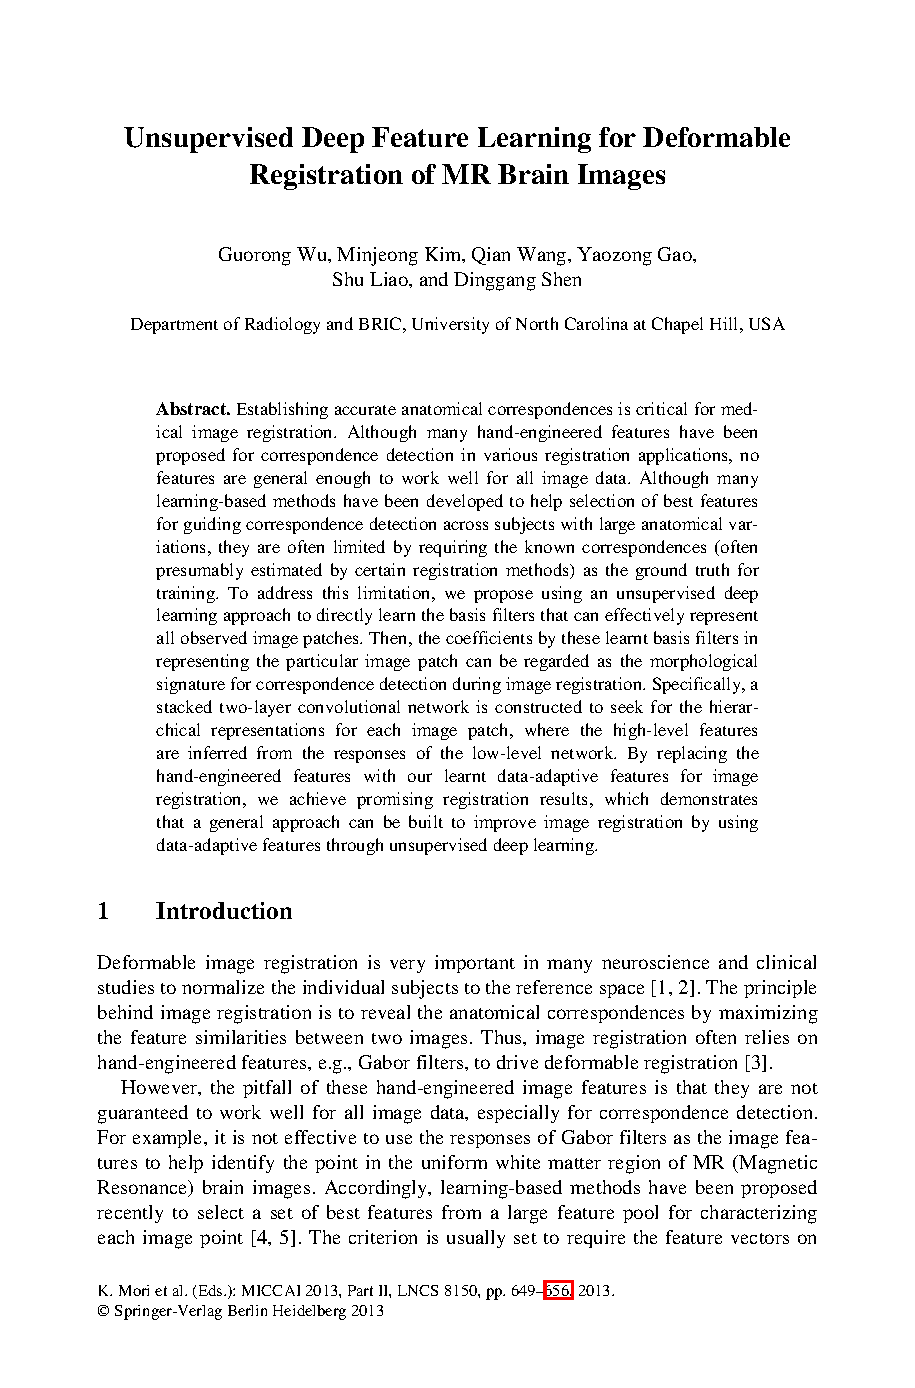
\includepdf[pages={-},scale=.9,pagecommand={}]{res/trans-english.pdf}

\chapter{外文资料的书面翻译}
最后再写吧


% vim: filetype=tex foldmethod=marker foldmarker=f{{{,f}}}

\end{appendix}

% 个人简历
%\include{data/resume}

\end{document}

% vim: filetype=tex foldmethod=marker foldmarker=f{{{,f}}}
